\section{Introduction}%


\begin{frame}
    \frametitle{Embedded Real-Time Control System}
    \framesubtitle<7>{Schedule}
    \begin{figure}[h]
        \centering
        \only<1>{\def \delta {0.15}
\def \circlesizecm {0.5cm}
\def \circleshiftcm {0.125cm}
\def \armlength {0.625}
\def \armwidthcm {0.1cm}
\def \bodywidthcm {0.5cm}

\begin{tikzpicture}
\tikzstyle{task} = [draw,thick,fill=white,align=center]
\tikzstyle{turbine} = [circle,ultra thick,draw,fill=white,minimum size=\circlesizecm,inner sep=0pt,outer sep=0pt]

%%% TASKS %%%

\node[task,opacity=0.3] (t1) at (-1.5+0*\delta,1.6-0*\delta) {\textcolor{white}{Task $\#3$} \\\textcolor{white}{\faFileCode[regular]}};
\node[task,opacity=0.6] (t2) at (-1.5+1*\delta,1.6-1*\delta) {\textcolor{white}{Task $\#2$} \\\textcolor{white}{\faFileCode[regular]}};
\node[task,opacity=1.0] (t3) at (-1.5+2*\delta,1.6-2*\delta) {Task $\#1$ \\\faFileCode[regular]};

\node[task,opacity=0.3] (ct1) at (1.5+0*\delta,1.6-0*\delta) {\textcolor{white}{Control Task $\#3$} \\\textcolor{white}{\faFileCode[regular]}};
\node[task,opacity=0.6] (ct2) at (1.5+1*\delta,1.6-1*\delta) {\textcolor{white}{Control Task $\#2$} \\\textcolor{white}{\faFileCode[regular]}};
\node[task,opacity=1.0] (ct3) at (1.5+2*\delta,1.6-2*\delta) {\textcolor{blue}{Control Task $\#1$} \\\textcolor{blue}{\faFileCode[regular]}};

%%% CYBER %%%

\node[thick, align=center] (rtos) at (-0.1,0.25) {Real-Time Operating System};
\node[thick, draw, align=center, rotate=90, text width=2.75cm] (hwi) at (4.1,0.87) {HW Interfaces};
\node[thick, fit=(rtos)(t1)(ct1)(ct3),draw,yshift=1.5mm,xshift=0.75mm] (sw) {};
\node[thick, draw, above left] (clock) at (sw.south east) {\faClock[regular]};
\node[thick, fit=(sw)(hwi), inner sep=7pt, draw] (hw) {};
\node[thick, above left, xshift=2.40cm, yshift=0.5mm] (hw-label) at (hw.south west) {Hardware};
\node[thick, draw, above right] (hwclock) at (hw.south west)  {\faClock[regular]};

%%% PHYSICAL %%%

\node[task, minimum width=2.125cm, minimum height=2.125cm] (phys) at (7.0,0.875) {};
% body
\node[
    draw,
    rounded corners=3pt,
    fill=black,
    minimum width=\bodywidthcm,
    minimum height=\bodywidthcm,
    name path=B] (body) at (phys) {};

% upper left turbine
\node[turbine, anchor=south east] (dronenw) at ([xshift=-\circleshiftcm, yshift=\circleshiftcm]body.north west) {};
\draw[name path=NW] ([yshift=-\armwidthcm]body.north west)..controls($(phys) + (-\armlength, \armlength)$)..([xshift=\armwidthcm]body.north west);
\tikzfillbetween [of=NW and B] {};
\draw[fill=black, rotate=75] (dronenw) ellipse (0.175cm and 0.025cm);
\draw[fill=black, rotate=165] (dronenw) ellipse (0.175cm and 0.025cm);
        
% upper right turbine
\node[turbine, anchor=south west] (dronene) at ([xshift=\circleshiftcm, yshift=\circleshiftcm]body.north east) {};
\draw[name path=NE] ([xshift=-\armwidthcm]body.north east)..controls($(phys) + (\armlength, \armlength)$)..([yshift=-\armwidthcm]body.north east);
\tikzfillbetween [of=NE and B] {};
\draw[fill=black, rotate=75] (dronene) ellipse (0.175cm and 0.025cm);
\draw[fill=black, rotate=165] (dronene) ellipse (0.175cm and 0.025cm);

% lower right turbine
\node[turbine, anchor=north west] (dronese) at ([xshift=\circleshiftcm, yshift=-\circleshiftcm]body.south east) {};
\draw[name path=SE] ([yshift=\armwidthcm]body.south east)..controls($(phys) + (\armlength, -\armlength)$)..([xshift=-\armwidthcm]body.south east);
\tikzfillbetween [of=SE and B] {};
\draw[fill=black, rotate=75] (dronese) ellipse (0.175cm and 0.025cm);
\draw[fill=black, rotate=165] (dronese) ellipse (0.175cm and 0.025cm);

% lower left turbine
\node[turbine, anchor=north east] (dronesw) at ([xshift=-\circleshiftcm, yshift=-\circleshiftcm]body.south west) {};
\draw[name path=SW] ([xshift=\armwidthcm]body.south west)..controls($(phys) + (-\armlength, -\armlength)$)..([yshift=\armwidthcm]body.south west);
\tikzfillbetween [of=SW and B] {};
\draw[fill=black, rotate=75] (dronesw) ellipse (0.175cm and 0.025cm);
\draw[fill=black, rotate=165] (dronesw) ellipse (0.175cm and 0.025cm);

% Clock
\node[task, above left] (time) at (phys.south east) {\faClock[regular]};

%%% ARROWS %%%

\draw[thick, -latex] ([yshift=0.65cm]hwi.south) to node[yshift=0.85cm,xshift=1mm,rotate=90] {\textcolor{blue}{Actuation}} ([yshift=0.65cm]phys.west);
\draw[thick, -latex] ([yshift=-0.65cm]phys.west) to node[yshift=-0.75cm,xshift=1mm,rotate=90] {\textcolor{blue}{Sensing}} ([yshift=-0.65cm]hwi.south);

\end{tikzpicture}
}%
        \only<2>{\def \delta {0.15}
\def \circlesizecm {0.5cm}
\def \circleshiftcm {0.125cm}
\def \armlength {0.625}
\def \armwidthcm {0.1cm}
\def \bodywidthcm {0.5cm}

\begin{tikzpicture}
\tikzstyle{task} = [draw,thick,fill=white,align=center]
\tikzstyle{turbine} = [circle,ultra thick,draw,fill=white,minimum size=\circlesizecm,inner sep=0pt,outer sep=0pt]

%%% TASKS %%%

\node[task,opacity=0.3] (t1) at (-1.5+0*\delta,1.6-0*\delta) {\textcolor{white}{Task $\#3$} \\\textcolor{white}{\faFileCode[regular]}};
\node[task,opacity=0.6] (t2) at (-1.5+1*\delta,1.6-1*\delta) {\textcolor{white}{Task $\#2$} \\\textcolor{white}{\faFileCode[regular]}};
\node[task,opacity=1.0] (t3) at (-1.5+2*\delta,1.6-2*\delta) {Task $\#1$ \\\faFileCode[regular]};

\node[task,opacity=0.3] (ct1) at (1.5+0*\delta,1.6-0*\delta) {\textcolor{white}{Control Task $\#3$} \\\textcolor{white}{\faFileCode[regular]}};
\node[task,opacity=0.6] (ct2) at (1.5+1*\delta,1.6-1*\delta) {\textcolor{white}{Control Task $\#2$} \\\textcolor{white}{\faFileCode[regular]}};
\node[task,opacity=1.0] (ct3) at (1.5+2*\delta,1.6-2*\delta) {Control Task $\#1$ \\\faFileCode[regular]};

%%% CYBER %%%

\node[thick, align=center] (rtos) at (-0.1,0.25) {Real-Time Operating System};
\node[thick, draw, align=center, rotate=90, text width=2.75cm] (hwi) at (4.1,0.87) {HW Interfaces};
\node[thick, fit=(rtos)(t1)(ct1)(ct3),draw,yshift=1.5mm,xshift=0.75mm] (sw) {};
\node[thick, draw, above left] (clock) at (sw.south east) {\faClock[regular]};
\node[thick, fit=(sw)(hwi), inner sep=7pt, draw] (hw) {};
\node[thick, above left, xshift=2.40cm, yshift=0.5mm] (hw-label) at (hw.south west) {Hardware};
\node[thick, draw, above right] (hwclock) at (hw.south west)  {\faClock[regular]};

%%% PHYSICAL %%%

\node[task, minimum width=2.125cm, minimum height=2.125cm, draw=hicolour] (phys) at (7.0,0.875) {};

% body
\node[
    draw,
    rounded corners=3pt,
    fill=black,
    minimum width=\bodywidthcm,
    minimum height=\bodywidthcm,
    name path=B] (body) at (phys) {};

% upper left turbine
\node[turbine, anchor=south east] (dronenw) at ([xshift=-\circleshiftcm, yshift=\circleshiftcm]body.north west) {};
\draw[name path=NW] ([yshift=-\armwidthcm]body.north west)..controls($(phys) + (-\armlength, \armlength)$)..([xshift=\armwidthcm]body.north west);
\tikzfillbetween [of=NW and B] {};
\draw[fill=black, rotate=75] (dronenw) ellipse (0.175cm and 0.025cm);
\draw[fill=black, rotate=165] (dronenw) ellipse (0.175cm and 0.025cm);
        
% upper right turbine
\node[turbine, anchor=south west] (dronene) at ([xshift=\circleshiftcm, yshift=\circleshiftcm]body.north east) {};
\draw[name path=NE] ([xshift=-\armwidthcm]body.north east)..controls($(phys) + (\armlength, \armlength)$)..([yshift=-\armwidthcm]body.north east);
\tikzfillbetween [of=NE and B] {};
\draw[fill=black, rotate=75] (dronene) ellipse (0.175cm and 0.025cm);
\draw[fill=black, rotate=165] (dronene) ellipse (0.175cm and 0.025cm);

% lower right turbine
\node[turbine, anchor=north west] (dronese) at ([xshift=\circleshiftcm, yshift=-\circleshiftcm]body.south east) {};
\draw[name path=SE] ([yshift=\armwidthcm]body.south east)..controls($(phys) + (\armlength, -\armlength)$)..([xshift=-\armwidthcm]body.south east);
\tikzfillbetween [of=SE and B] {};
\draw[fill=black, rotate=75] (dronese) ellipse (0.175cm and 0.025cm);
\draw[fill=black, rotate=165] (dronese) ellipse (0.175cm and 0.025cm);

% lower left turbine
\node[turbine, anchor=north east] (dronesw) at ([xshift=-\circleshiftcm, yshift=-\circleshiftcm]body.south west) {};
\draw[name path=SW] ([xshift=\armwidthcm]body.south west)..controls($(phys) + (-\armlength, -\armlength)$)..([yshift=\armwidthcm]body.south west);
\tikzfillbetween [of=SW and B] {};
\draw[fill=black, rotate=75] (dronesw) ellipse (0.175cm and 0.025cm);
\draw[fill=black, rotate=165] (dronesw) ellipse (0.175cm and 0.025cm);

% Clock
{\color{hicolour}\node[task, above left] (time) at (phys.south east) {\faClock[regular]};}

{\color{hicolour}\node[] (phystmp) at ([yshift=-0.25cm]phys.south) {Plant};}

%%% ARROWS %%%

\draw[thick, -latex] ([yshift=0.65cm]hwi.south) to node[yshift=0.85cm,xshift=1mm,rotate=90] {Actuation} ([yshift=0.65cm]phys.west);
\draw[thick, -latex] ([yshift=-0.65cm]phys.west) to node[yshift=-0.75cm,xshift=1mm,rotate=90] {Sensing} ([yshift=-0.65cm]hwi.south);

\end{tikzpicture}
}%
        \only<3>{\def \delta {0.15}

\begin{tikzpicture}
\tikzstyle{task} = [draw, fill=white,align=center]

%%%%%%%%%%%
%%% CPS %%%
%%%%%%%%%%%

%%% TASKS %%%

\node[task,] (t1) at (-2+0*\delta,1.6-0*\delta) {Task $\#1$ \\\faFileCode[regular]};
\node[task,] (t2) at (-2+1*\delta,1.6-1*\delta) {Task $\#2$ \\\faFileCode[regular]};
\node[task,] (t3) at (-2+2*\delta,1.6-2*\delta) {Task $\#3$ \\\faFileCode[regular]};

\node[task,] (ct1) at (1+0*\delta,1.6-0*\delta) {Control-Task $\#1$ \\\faFileCode[regular]};
\node[task,] (ct2) at (1+1*\delta,1.6-1*\delta) {Control-Task $\#2$ \\\faFileCode[regular]};
\node[task,] (ct3) at (1+2*\delta,1.6-2*\delta) {Control-Task $\#3$ \\\faFileCode[regular]};

%%% CYBER %%%

\node[align=center] (rtos) at (-0.2,0.15)  {Real-Time Operating System};
\node[draw, align=center, rotate=90, text width=3.0cm] (hw)   at (3.35,0.775) {HW interfaces};
\node[fit=(rtos)(t1)(ct1)(ct3),draw,yshift=1.5mm] (sw) {};
\node[draw, above left] (clock) at (sw.south east)  {\faClock[regular]};
{\color{lqgcolour}\node[thick, fit=(sw)(hw),draw] (board) {};}
{\color{lqgcolour}\node[above left, xshift=1.8cm] (borad-label) at (board.south west) {Board};}
{\color{lqgcolour}\node[draw, above right] (clockboard) at (board.south west)  {\faClock[regular]};}

%%% PHYSICAL %%%

\node[thick, draw ,align=center] (phys) at (6,0.775) {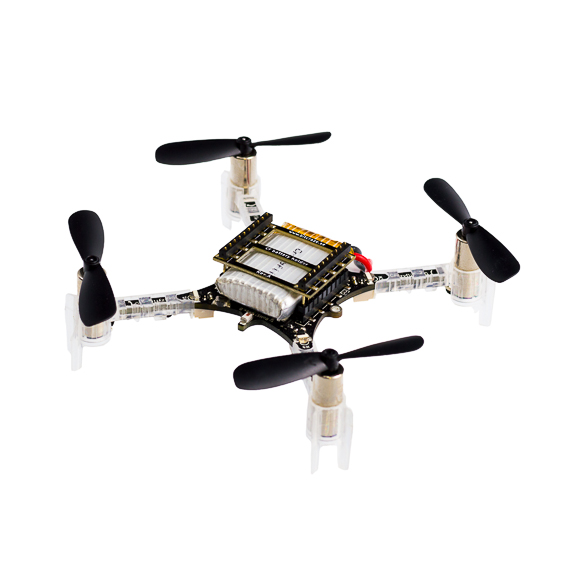
\includegraphics[scale=0.4]{figs/topic/crazyflie.jpg}};
\node[draw, above left] (time) at (phys.south east)  {\faClock[regular]};

%%% ARROWS %%%

\draw[-latex] ([yshift=0.65cm]hw.south) to node[yshift=0.85cm,rotate=90]{actuation} ([yshift=0.65cm]phys.west);
\draw[-latex] ([yshift=-0.65cm]phys.west) to node[yshift=-0.85cm, rotate=90]{sensing} ([yshift=-0.65cm]hw.south);

\end{tikzpicture}
}%
        \only<4>{\def \delta {0.15}
\def \circlesizecm {0.5cm}
\def \circleshiftcm {0.125cm}
\def \armlength {0.625}
\def \armwidthcm {0.1cm}
\def \bodywidthcm {0.5cm}

\begin{tikzpicture}
\tikzstyle{task} = [draw,thick,fill=white,align=center]
\tikzstyle{turbine} = [circle,ultra thick,draw,fill=white,minimum size=\circlesizecm,inner sep=0pt,outer sep=0pt]

%%% TASKS %%%

\node[task,opacity=0.3] (t1) at (-1.5+0*\delta,1.6-0*\delta) {\textcolor{white}{Task $\#3$} \\\textcolor{white}{\faFileCode[regular]}};
\node[task,opacity=0.6] (t2) at (-1.5+1*\delta,1.6-1*\delta) {\textcolor{white}{Task $\#2$} \\\textcolor{white}{\faFileCode[regular]}};
\node[task,opacity=1.0] (t3) at (-1.5+2*\delta,1.6-2*\delta) {Task $\#1$ \\\faFileCode[regular]};

\node[task,opacity=0.3] (ct1) at (1.5+0*\delta,1.6-0*\delta) {\textcolor{white}{Control Task $\#3$} \\\textcolor{white}{\faFileCode[regular]}};
\node[task,opacity=0.6] (ct2) at (1.5+1*\delta,1.6-1*\delta) {\textcolor{white}{Control Task $\#2$} \\\textcolor{white}{\faFileCode[regular]}};
\node[task,opacity=1.0] (ct3) at (1.5+2*\delta,1.6-2*\delta) {\textcolor{hicolour}{Control Task $\#1$} \\\textcolor{hicolour}{\faFileCode[regular]}};

%%% CYBER %%%

\node[thick, align=center] (rtos) at (-0.1,0.25) {Real-Time Operating System};
\node[thick, draw, align=center, rotate=90, text width=2.75cm] (hwi) at (4.1,0.87) {HW Interfaces};
\node[thick, fit=(rtos)(t1)(ct1)(ct3),draw,yshift=1.5mm,xshift=0.75mm] (sw) {};
\node[thick, draw, above left] (clock) at (sw.south east) {\faClock[regular]};
\node[thick, fit=(sw)(hwi), inner sep=7pt, draw] (hw) {};
\node[thick, above left, xshift=2.40cm, yshift=0.5mm] (hw-label) at (hw.south west) {Hardware};
\node[thick, draw, above right] (hwclock) at (hw.south west)  {\faClock[regular]};

%%% PHYSICAL %%%

\node[task, minimum width=2.125cm, minimum height=2.125cm] (phys) at (7.0,0.875) {};
% body
\node[
    draw,
    rounded corners=3pt,
    fill=black,
    minimum width=\bodywidthcm,
    minimum height=\bodywidthcm,
    name path=B] (body) at (phys) {};

% upper left turbine
\node[turbine, anchor=south east] (dronenw) at ([xshift=-\circleshiftcm, yshift=\circleshiftcm]body.north west) {};
\draw[name path=NW] ([yshift=-\armwidthcm]body.north west)..controls($(phys) + (-\armlength, \armlength)$)..([xshift=\armwidthcm]body.north west);
\tikzfillbetween [of=NW and B] {};
\draw[fill=black, rotate=75] (dronenw) ellipse (0.175cm and 0.025cm);
\draw[fill=black, rotate=165] (dronenw) ellipse (0.175cm and 0.025cm);
        
% upper right turbine
\node[turbine, anchor=south west] (dronene) at ([xshift=\circleshiftcm, yshift=\circleshiftcm]body.north east) {};
\draw[name path=NE] ([xshift=-\armwidthcm]body.north east)..controls($(phys) + (\armlength, \armlength)$)..([yshift=-\armwidthcm]body.north east);
\tikzfillbetween [of=NE and B] {};
\draw[fill=black, rotate=75] (dronene) ellipse (0.175cm and 0.025cm);
\draw[fill=black, rotate=165] (dronene) ellipse (0.175cm and 0.025cm);

% lower right turbine
\node[turbine, anchor=north west] (dronese) at ([xshift=\circleshiftcm, yshift=-\circleshiftcm]body.south east) {};
\draw[name path=SE] ([yshift=\armwidthcm]body.south east)..controls($(phys) + (\armlength, -\armlength)$)..([xshift=-\armwidthcm]body.south east);
\tikzfillbetween [of=SE and B] {};
\draw[fill=black, rotate=75] (dronese) ellipse (0.175cm and 0.025cm);
\draw[fill=black, rotate=165] (dronese) ellipse (0.175cm and 0.025cm);

% lower left turbine
\node[turbine, anchor=north east] (dronesw) at ([xshift=-\circleshiftcm, yshift=-\circleshiftcm]body.south west) {};
\draw[name path=SW] ([xshift=\armwidthcm]body.south west)..controls($(phys) + (-\armlength, -\armlength)$)..([yshift=\armwidthcm]body.south west);
\tikzfillbetween [of=SW and B] {};
\draw[fill=black, rotate=75] (dronesw) ellipse (0.175cm and 0.025cm);
\draw[fill=black, rotate=165] (dronesw) ellipse (0.175cm and 0.025cm);

% Clock
\node[task, above left] (time) at (phys.south east) {\faClock[regular]};

%%% ARROWS %%%

{\color{hicolour}\draw[thick, -latex] ([yshift=0.65cm]hwi.south) to node[yshift=0.85cm,xshift=1mm,rotate=90] {\phantom{Actuation}} ([yshift=0.65cm]phys.west);}
{\color{red}\draw[thick, -latex] ([yshift=-0.65cm]phys.west) to node[yshift=-0.75cm,xshift=1mm,rotate=90] {\phantom{Sensing}} ([yshift=-0.65cm]hwi.south);}

%%% Packets
\node (packetS) at ([xshift=-0.25cm, yshift=-0.4cm]phys.west) {\textcolor{red}{\faBox}};

\node (packetA) at ([xshift=0.5cm, yshift=0.9cm]hwi.south) {\textcolor{hicolour!85!white}{\faBox}};


\end{tikzpicture}
}%
        \only<5>{\def \delta {0.15}
\def \circlesizecm {0.5cm}
\def \circleshiftcm {0.125cm}
\def \armlength {0.625}
\def \armwidthcm {0.1cm}
\def \bodywidthcm {0.5cm}

\begin{tikzpicture}
\tikzstyle{task} = [draw,thick,fill=white,align=center]
\tikzstyle{turbine} = [circle,ultra thick,draw,fill=white,minimum size=\circlesizecm,inner sep=0pt,outer sep=0pt]

%%% TASKS %%%

\node[task,opacity=0.3] (t1) at (-1.5+0*\delta,1.6-0*\delta) {\textcolor{white}{Task $\#3$} \\\textcolor{white}{\faFileCode[regular]}};
\node[task,opacity=0.6] (t2) at (-1.5+1*\delta,1.6-1*\delta) {\textcolor{white}{Task $\#2$} \\\textcolor{white}{\faFileCode[regular]}};
\node[task,opacity=1.0] (t3) at (-1.5+2*\delta,1.6-2*\delta) {Task $\#1$ \\\faFileCode[regular]};

\node[task,opacity=0.3] (ct1) at (1.5+0*\delta,1.6-0*\delta) {\textcolor{white}{Control Task $\#3$} \\\textcolor{white}{\faFileCode[regular]}};
\node[task,opacity=0.6] (ct2) at (1.5+1*\delta,1.6-1*\delta) {\textcolor{white}{Control Task $\#2$} \\\textcolor{white}{\faFileCode[regular]}};
\node[task,opacity=1.0] (ct3) at (1.5+2*\delta,1.6-2*\delta) {Control Task $\#1$ \\\faFileCode[regular]};

%%% CYBER %%%

{\color{lqgcolour}\node[thick, align=center] (rtos) at (-0.1,0.25) {Real-Time Operating System};}
\node[thick, draw, align=center, rotate=90, text width=2.75cm] (hwi) at (4.1,0.87) {HW Interfaces};
{\color{lqgcolour}\node[thick, fit=(rtos)(t1)(ct1)(ct3),draw,yshift=1.5mm,xshift=0.75mm] (sw) {};}
{\color{lqgcolour}\node[thick, draw, above left] (clock) at (sw.south east) {\faClock[regular]};}
\node[thick, fit=(sw)(hwi), inner sep=7pt, draw] (hw) {};
\node[thick, above left, xshift=2.40cm, yshift=0.5mm] (hw-label) at (hw.south west) {Hardware};
\node[thick, draw, above right] (hwclock) at (hw.south west)  {\faClock[regular]};

%%% PHYSICAL %%%

\node[task, minimum width=2.125cm, minimum height=2.125cm] (phys) at (7.0,0.875) {};
% body
\node[
    draw,
    rounded corners=3pt,
    fill=black,
    minimum width=\bodywidthcm,
    minimum height=\bodywidthcm,
    name path=B] (body) at (phys) {};

% upper left turbine
\node[turbine, anchor=south east] (dronenw) at ([xshift=-\circleshiftcm, yshift=\circleshiftcm]body.north west) {};
\draw[name path=NW] ([yshift=-\armwidthcm]body.north west)..controls($(phys) + (-\armlength, \armlength)$)..([xshift=\armwidthcm]body.north west);
\tikzfillbetween [of=NW and B] {};
\draw[fill=black, rotate=75] (dronenw) ellipse (0.175cm and 0.025cm);
\draw[fill=black, rotate=165] (dronenw) ellipse (0.175cm and 0.025cm);
        
% upper right turbine
\node[turbine, anchor=south west] (dronene) at ([xshift=\circleshiftcm, yshift=\circleshiftcm]body.north east) {};
\draw[name path=NE] ([xshift=-\armwidthcm]body.north east)..controls($(phys) + (\armlength, \armlength)$)..([yshift=-\armwidthcm]body.north east);
\tikzfillbetween [of=NE and B] {};
\draw[fill=black, rotate=75] (dronene) ellipse (0.175cm and 0.025cm);
\draw[fill=black, rotate=165] (dronene) ellipse (0.175cm and 0.025cm);

% lower right turbine
\node[turbine, anchor=north west] (dronese) at ([xshift=\circleshiftcm, yshift=-\circleshiftcm]body.south east) {};
\draw[name path=SE] ([yshift=\armwidthcm]body.south east)..controls($(phys) + (\armlength, -\armlength)$)..([xshift=-\armwidthcm]body.south east);
\tikzfillbetween [of=SE and B] {};
\draw[fill=black, rotate=75] (dronese) ellipse (0.175cm and 0.025cm);
\draw[fill=black, rotate=165] (dronese) ellipse (0.175cm and 0.025cm);

% lower left turbine
\node[turbine, anchor=north east] (dronesw) at ([xshift=-\circleshiftcm, yshift=-\circleshiftcm]body.south west) {};
\draw[name path=SW] ([xshift=\armwidthcm]body.south west)..controls($(phys) + (-\armlength, -\armlength)$)..([yshift=\armwidthcm]body.south west);
\tikzfillbetween [of=SW and B] {};
\draw[fill=black, rotate=75] (dronesw) ellipse (0.175cm and 0.025cm);
\draw[fill=black, rotate=165] (dronesw) ellipse (0.175cm and 0.025cm);

% Clock
\node[task, above left] (time) at (phys.south east) {\faClock[regular]};

%%% ARROWS %%%

\draw[thick, -latex] ([yshift=0.65cm]hwi.south) to node[yshift=0.85cm,xshift=1mm,rotate=90] {Actuation} ([yshift=0.65cm]phys.west);
\draw[thick, -latex] ([yshift=-0.65cm]phys.west) to node[yshift=-0.75cm,xshift=1mm,rotate=90] {Sensing} ([yshift=-0.65cm]hwi.south);

\end{tikzpicture}
}%
        \only<6>{\def \delta {0.15}
\def \circlesizecm {0.5cm}
\def \circleshiftcm {0.125cm}
\def \armlength {0.625}
\def \armwidthcm {0.1cm}
\def \bodywidthcm {0.5cm}

\begin{tikzpicture}
\tikzstyle{task} = [draw,thick,fill=white,align=center]
\tikzstyle{turbine} = [circle,ultra thick,draw,fill=white,minimum size=\circlesizecm,inner sep=0pt,outer sep=0pt]
\tikzstyle{circleconn} = [draw, fill=white, thick, circle, scale=0.5]

%%% TASKS %%%

\begin{scope}[on background layer]
    \tikzstyle{task} = [draw,thick,fill=white,align=center]
    \tikzstyle{turbine} = [circle,ultra thick,draw,fill=white,minimum size=\circlesizecm,inner sep=0pt,outer sep=0pt]

    %%% TASKS %%%

    \node[task,opacity=0.3] (t1) at (-1.5+0*\delta,1.6-0*\delta) {\textcolor{white}{Task $\#3$} \\\textcolor{white}{\faFileCode[regular]}};
    \node[task,opacity=0.6] (t2) at (-1.5+1*\delta,1.6-1*\delta) {\textcolor{white}{Task $\#2$} \\\textcolor{white}{\faFileCode[regular]}};
    \node[task,opacity=1.0] (t3) at (-1.5+2*\delta,1.6-2*\delta) {Task $\#1$ \\\faFileCode[regular]};

    \node[task,opacity=0.3] (ct1) at (1.5+0*\delta,1.6-0*\delta) {\textcolor{white}{Control Task $\#3$} \\\textcolor{white}{\faFileCode[regular]}};
    \node[task,opacity=0.6] (ct2) at (1.5+1*\delta,1.6-1*\delta) {\textcolor{white}{Control Task $\#2$} \\\textcolor{white}{\faFileCode[regular]}};
    \node[task,opacity=1.0] (ct3) at (1.5+2*\delta,1.6-2*\delta) {Control Task $\#1$ \\\faFileCode[regular]};

    %%% CYBER %%%

    \node[thick, align=center] (rtos) at (-0.1,0.25) {Real-Time Operating System};
    \node[thick, draw, align=center, rotate=90, text width=2.75cm] (hwi) at (4.1,0.87) {HW Interfaces};
    \node[thick, fit=(rtos)(t1)(ct1)(ct3),draw,yshift=1.5mm,xshift=0.75mm] (sw) {};
    \node[thick, draw, above left] (clock) at (sw.south east) {\faClock[regular]};
    \node[thick, fit=(sw)(hwi), inner sep=7pt, draw] (hw) {};
    \node[thick, above left, xshift=2.40cm, yshift=0.5mm] (hw-label) at (hw.south west) {Hardware};
    \node[thick, draw, above right] (hwclock) at (hw.south west)  {\faClock[regular]};

    %%% PHYSICAL %%%

    \node[task, minimum width=2.125cm, minimum height=2.125cm] (phys) at (7.0,0.875) {};
    % body
    \node[
        draw,
        rounded corners=3pt,
        fill=black,
        minimum width=\bodywidthcm,
        minimum height=\bodywidthcm,
        name path=B] (body) at (phys) {};

    % upper left turbine
    \node[turbine, anchor=south east] (dronenw) at ([xshift=-\circleshiftcm, yshift=\circleshiftcm]body.north west) {};
    \draw[name path=NW] ([yshift=-\armwidthcm]body.north west)..controls($(phys) + (-\armlength, \armlength)$)..([xshift=\armwidthcm]body.north west);
    \tikzfillbetween [of=NW and B] {};
    \draw[fill=black, rotate=75] (dronenw) ellipse (0.175cm and 0.025cm);
    \draw[fill=black, rotate=165] (dronenw) ellipse (0.175cm and 0.025cm);

    % upper right turbine
    \node[turbine, anchor=south west] (dronene) at ([xshift=\circleshiftcm, yshift=\circleshiftcm]body.north east) {};
    \draw[name path=NE] ([xshift=-\armwidthcm]body.north east)..controls($(phys) + (\armlength, \armlength)$)..([yshift=-\armwidthcm]body.north east);
    \tikzfillbetween [of=NE and B] {};
    \draw[fill=black, rotate=75] (dronene) ellipse (0.175cm and 0.025cm);
    \draw[fill=black, rotate=165] (dronene) ellipse (0.175cm and 0.025cm);

    % lower right turbine
    \node[turbine, anchor=north west] (dronese) at ([xshift=\circleshiftcm, yshift=-\circleshiftcm]body.south east) {};
    \draw[name path=SE] ([yshift=\armwidthcm]body.south east)..controls($(phys) + (\armlength, -\armlength)$)..([xshift=-\armwidthcm]body.south east);
    \tikzfillbetween [of=SE and B] {};
    \draw[fill=black, rotate=75] (dronese) ellipse (0.175cm and 0.025cm);
    \draw[fill=black, rotate=165] (dronese) ellipse (0.175cm and 0.025cm);

    % lower left turbine
    \node[turbine, anchor=north east] (dronesw) at ([xshift=-\circleshiftcm, yshift=-\circleshiftcm]body.south west) {};
    \draw[name path=SW] ([xshift=\armwidthcm]body.south west)..controls($(phys) + (-\armlength, -\armlength)$)..([yshift=\armwidthcm]body.south west);
    \tikzfillbetween [of=SW and B] {};
    \draw[fill=black, rotate=75] (dronesw) ellipse (0.175cm and 0.025cm);
    \draw[fill=black, rotate=165] (dronesw) ellipse (0.175cm and 0.025cm);

    % Clock
    \node[task, above left] (time) at (phys.south east) {\faClock[regular]};

    %%% ARROWS %%%

    \draw[thick, -latex] ([yshift=0.65cm]hwi.south) to node[yshift=0.85cm,xshift=1mm,rotate=90] {} ([yshift=0.65cm]phys.west);
    \draw[thick, -latex] ([yshift=-0.65cm]phys.west) to node[yshift=-0.75cm,xshift=1mm,rotate=90] {} ([yshift=-0.65cm]hwi.south);

\end{scope}


%%% ZOOM %%%

% Tasks
\node[task] (vt1) at (-1.3+0*12*\delta,1.0) {Task $\#1$ \\\faFileCode[regular]};
\node[task] (vt2) at (-1.3+1*12*\delta,1.0) {Task $\#2$ \\\faFileCode[regular]};
\node[]           at (-1.3+1.75*12*\delta,1.0) {$\cdots$};
\node[task] (vtn) at (-1.3+2.5*12*\delta,1.0) {Task $\#N$ \\\faFileCode[regular]};

\node[circleconn] (c1) at ($(vt1)+(0,-0.75)$) {};
\draw[thick] (c1.north) to (vt1.south);
\node[circleconn] (c2) at ($(vt2)+(0,-0.75)$) {};
\draw[thick] (c2.north) to (vt2.south);
\node[circleconn] (cn) at ($(vtn)+(0,-0.75)$) {};
\draw[thick] (cn.north) to (vtn.south);

% CPU
\node[task, minimum width=4.0cm, minimum height=2.0cm] (cpu) at (-0.9+1.5*10*\delta,-2.65) {};
\node[task, minimum width=2.0cm, minimum height=0.6cm, rotate=90] (cache) at ([xshift=-0.3cm]cpu.east) {Cache};

% Cores
\node[task, opacity=0.7, minimum width=1.8cm, minimum height=0.6cm, rotate=90] (core1) at ([xshift=0.5cm]cpu.west) {Core $\#1$};
\node[task, opacity=0.7, minimum width=1.8cm, minimum height=0.6cm, rotate=90] (core2) at ([xshift=0.5cm]core1.south) {Core $\#2$};
\node[task, opacity=0.7, minimum width=1.8cm, minimum height=0.6cm, rotate=90] (coreM) at ([xshift=-0.5cm]cache.north) {Core $\#M$};
\node[opacity=0.7] at ([xshift=-0.5cm]coreM.north) {$\cdots$};
\node[rotate=90, above] at (cpu.west) {CPU};

% Memory
\node[task, minimum width=1.8cm, minimum height=0.6cm, rotate=90] (mem) at (-1.3+4*10*\delta,-2.65) {Memory};

% Cache lines
\node[circleconn] (ccache) at ([xshift=0.25cm]cache.south) {};
\draw[thick] (cache.south) to (ccache.west);

\draw[thick, -latex] (ccache.east) to ([yshift=-2mm]mem.north);
\draw[thick, dashed, -latex, opacity=0.3] (ccache.east) to ([yshift=5mm]mem.north);
\draw[thick, dashed, -latex, opacity=0.3] (ccache.east) to ([yshift=-6mm]mem.north);

% HW interfaces
\node[task, minimum width=2.3cm, minimum height=0.6cm, rotate=90] (gpio) at (-1.3+4*10*\delta,0.15) {I/O Interface};

% Lines into memory
\node[circleconn] (cgpio) at ([yshift=-0.38cm]gpio.west) {};
\draw[thick] (gpio.west) to (cgpio.north);
\draw[thick] (cgpio.south) to (mem.east);


% Background 
\begin{scope}[on background layer]
    \node[ultra thick, fill=white, fit=(vt1)(vtn)(cpu)(mem),draw,inner sep=4pt] (vhw) {};
    %\draw[thick, dashed] ([yshift=-0.35cm]vhw.west) to ([yshift=-0.35cm,xshift=-1.0cm]vhw.east);
    \draw[thick, dashed] ([yshift=-0.35cm]vhw.west) to ([yshift=-0.35cm]vhw.east);
    \draw[thick, dashed] ([xshift=2.75cm]vhw.south) to ([xshift=2.75cm]vhw.north);
\end{scope}

\draw[thick, dashed] (hw.south west) to (vhw.south west);
\draw[thick, dashed] (hw.north west) to (vhw.north west);
\draw[thick, dashed] (hw.north east) to (vhw.north east);

% Scheduler
\node[task, minimum width=4cm, minimum height=0.6cm] (sched) at (-0.9+1.5*10*\delta,-0.85) {Scheduler};
\node[circleconn] (csched) at ($(sched)+(0,0.55)$) {};
\draw[thick] (csched.south) to (sched.north);

\node[circleconn] (ccpu) at ($(sched)+(0,-0.55)$) {};
\draw[thick] (sched.south) to (ccpu.north);

\draw[thick, -latex] (csched.north) to (c2.south);
\draw[thick, dashed, -latex, opacity=0.3] (csched.north) to (c1.south);
\draw[thick, dashed, -latex, opacity=0.3] (csched.north) to (cn.south);

\draw[thick, -latex] (ccpu.south) to (core1.east);
\draw[thick, dashed, -latex, opacity=0.3] (ccpu.south) to (core2.east);
\draw[thick, dashed, -latex, opacity=0.3] (ccpu.south) to (coreM.east);

\end{tikzpicture}
}%
        \only<7>{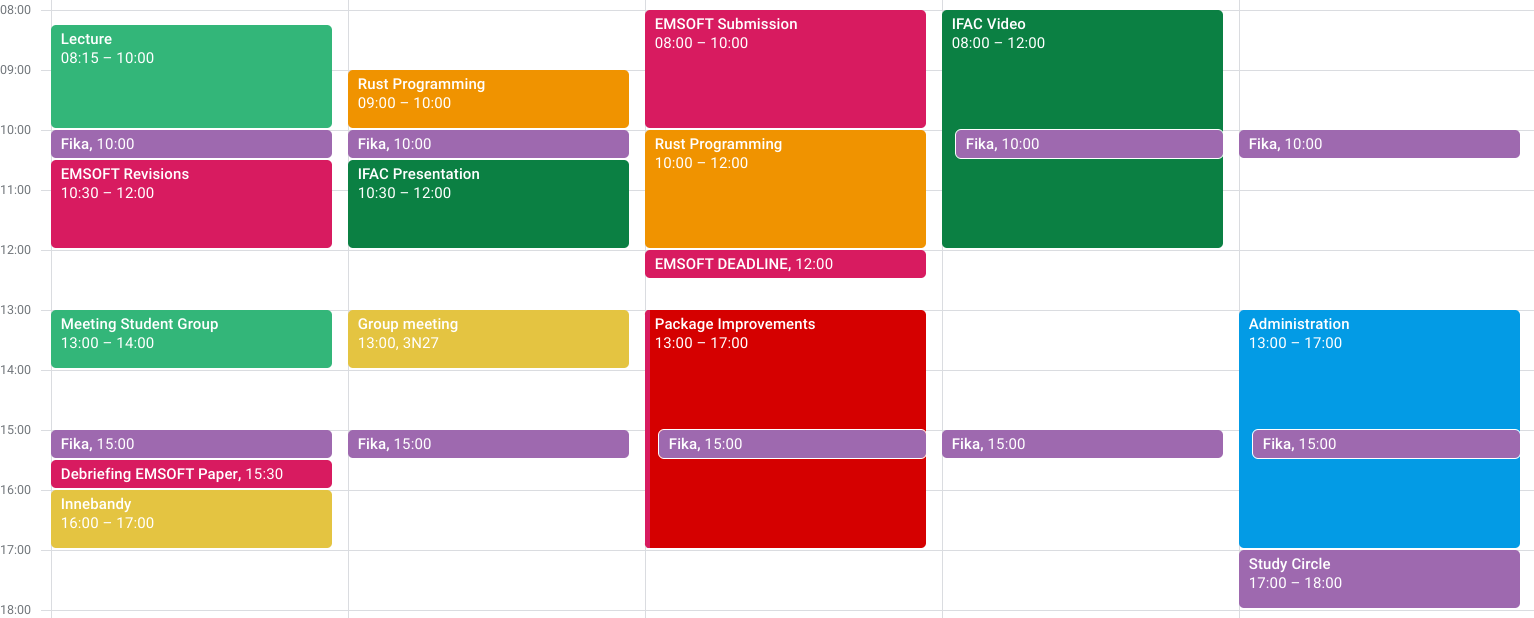
\includegraphics[width=1.0\textwidth]{figs/topic/schedule.png}}%
        \only<8>{\def \delta {0.15}

\begin{tikzpicture}
\tikzstyle{task} = [draw, fill=white,align=center]

%%%%%%%%%%%
%%% CPS %%%
%%%%%%%%%%%

%%% TASKS %%%

\node[task,] (t1) at (-2+0*\delta,1.6-0*\delta) {Task $\#1$ \\\faFileCode[regular]};
\node[task,] (t2) at (-2+1*\delta,1.6-1*\delta) {Task $\#2$ \\\faFileCode[regular]};
\node[task,] (t3) at (-2+2*\delta,1.6-2*\delta) {Task $\#3$ \\\faFileCode[regular]};

{\color{lqgcolour}\node[task,] (ct1) at (1+0*\delta,1.6-0*\delta) {Control-Task $\#1$ \\\faFileCode[regular]};}
{\color{lqgcolour}\node[task,] (ct2) at (1+1*\delta,1.6-1*\delta) {Control-Task $\#2$ \\\faFileCode[regular]};}
{\color{lqgcolour}\node[task,] (ct3) at (1+2*\delta,1.6-2*\delta) {Control-Task $\#3$ \\\faFileCode[regular]};}

%%% CYBER %%%

\node[align=center] (rtos) at (-0.2,0.15)  {Real-Time Operating System};
\node[draw, align=center, rotate=90, text width=3.0cm] (hw)   at (3.35,0.775) {HW interfaces};
\node[fit=(rtos)(t1)(ct1)(ct3),draw,yshift=1.5mm] (sw) {};
\node[draw, above left] (clock) at (sw.south east)  {\faClock[regular]};
\node[thick, fit=(sw)(hw),draw] (board) {};
\node[above left, xshift=1.8cm] (borad-label) at (board.south west) {Board};
\node[draw, above right] (clockboard) at (board.south west)  {\faClock[regular]};

%%% PHYSICAL %%%

\node[thick, draw ,align=center] (phys) at (6,0.775) {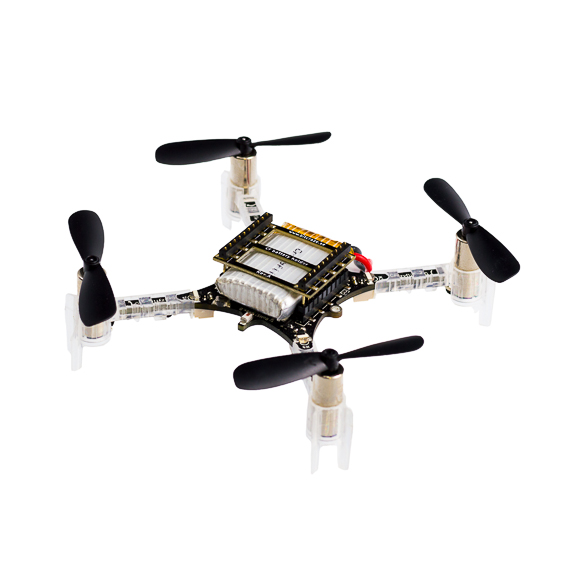
\includegraphics[scale=0.4]{figs/topic/crazyflie.jpg}};
\node[draw, above left] (time) at (phys.south east)  {\faClock[regular]};

%%% ARROWS %%%

\draw[-latex] ([yshift=0.65cm]hw.south) to node[yshift=0.85cm,rotate=90]{actuation} ([yshift=0.65cm]phys.west);
\draw[-latex] ([yshift=-0.65cm]phys.west) to node[yshift=-0.85cm, rotate=90]{sensing} ([yshift=-0.65cm]hw.south);

\end{tikzpicture}
}%
        \only<9>{\def \delta {0.15}
\def \circlesizecm {0.5cm}
\def \circleshiftcm {0.125cm}
\def \armlength {0.625}
\def \armwidthcm {0.1cm}
\def \bodywidthcm {0.5cm}

\begin{tikzpicture}
\tikzstyle{task} = [draw,thick,fill=white,align=center]
\tikzstyle{turbine} = [circle,ultra thick,draw,fill=white,minimum size=\circlesizecm,inner sep=0pt,outer sep=0pt]

%%% TASKS %%%

\node[task,opacity=0.3] (t1) at (-1.5+0*\delta,1.6-0*\delta) {\textcolor{white}{Task $\#3$} \\\textcolor{white}{\faFileCode[regular]}};
\node[task,opacity=0.6] (t2) at (-1.5+1*\delta,1.6-1*\delta) {\textcolor{white}{Task $\#2$} \\\textcolor{white}{\faFileCode[regular]}};
\node[task,opacity=1.0] (t3) at (-1.5+2*\delta,1.6-2*\delta) {Task $\#1$ \\\faFileCode[regular]};

{\color{lqgcolour}\node[task,opacity=0.3] (ct1) at (1.5+0*\delta,1.6-0*\delta) {\textcolor{white}{Control Task $\#3$} \\\textcolor{white}{\faFileCode[regular]}};}
{\color{lqgcolour}\node[task,opacity=0.6] (ct2) at (1.5+1*\delta,1.6-1*\delta) {\textcolor{white}{Control Task $\#2$} \\\textcolor{white}{\faFileCode[regular]}};}
{\color{lqgcolour}\node[task,opacity=1.0] (ct3) at (1.5+2*\delta,1.6-2*\delta) {Control Task $\#1$ \\\faFileCode[regular]};}

%%% CYBER %%%

\node[thick, align=center] (rtos) at (-0.1,0.25) {Real-Time Operating System};
\node[thick, draw, align=center, rotate=90, text width=2.75cm] (hwi) at (4.1,0.87) {HW Interfaces};
\node[thick, fit=(rtos)(t1)(ct1)(ct3),draw,yshift=1.5mm,xshift=0.75mm] (sw) {};
\node[thick, draw, above left] (clock) at (sw.south east) {\faClock[regular]};
\node[thick, fit=(sw)(hwi), inner sep=7pt, draw] (hw) {};
\node[thick, above left, xshift=2.40cm, yshift=0.5mm] (hw-label) at (hw.south west) {Hardware};
\node[thick, draw, above right] (hwclock) at (hw.south west)  {\faClock[regular]};

%%% PHYSICAL %%%

\node[task, minimum width=2.125cm, minimum height=2.125cm] (phys) at (7.0,0.875) {};
% body
\node[
    draw,
    rounded corners=3pt,
    fill=black,
    minimum width=\bodywidthcm,
    minimum height=\bodywidthcm,
    name path=B] (body) at (phys) {};

% upper left turbine
\node[turbine, anchor=south east] (dronenw) at ([xshift=-\circleshiftcm, yshift=\circleshiftcm]body.north west) {};
\draw[name path=NW] ([yshift=-\armwidthcm]body.north west)..controls($(phys) + (-\armlength, \armlength)$)..([xshift=\armwidthcm]body.north west);
\tikzfillbetween [of=NW and B] {};
\draw[fill=black, rotate=75] (dronenw) ellipse (0.175cm and 0.025cm);
\draw[fill=black, rotate=165] (dronenw) ellipse (0.175cm and 0.025cm);
        
% upper right turbine
\node[turbine, anchor=south west] (dronene) at ([xshift=\circleshiftcm, yshift=\circleshiftcm]body.north east) {};
\draw[name path=NE] ([xshift=-\armwidthcm]body.north east)..controls($(phys) + (\armlength, \armlength)$)..([yshift=-\armwidthcm]body.north east);
\tikzfillbetween [of=NE and B] {};
\draw[fill=black, rotate=75] (dronene) ellipse (0.175cm and 0.025cm);
\draw[fill=black, rotate=165] (dronene) ellipse (0.175cm and 0.025cm);

% lower right turbine
\node[turbine, anchor=north west] (dronese) at ([xshift=\circleshiftcm, yshift=-\circleshiftcm]body.south east) {};
\draw[name path=SE] ([yshift=\armwidthcm]body.south east)..controls($(phys) + (\armlength, -\armlength)$)..([xshift=-\armwidthcm]body.south east);
\tikzfillbetween [of=SE and B] {};
\draw[fill=black, rotate=75] (dronese) ellipse (0.175cm and 0.025cm);
\draw[fill=black, rotate=165] (dronese) ellipse (0.175cm and 0.025cm);

% lower left turbine
\node[turbine, anchor=north east] (dronesw) at ([xshift=-\circleshiftcm, yshift=-\circleshiftcm]body.south west) {};
\draw[name path=SW] ([xshift=\armwidthcm]body.south west)..controls($(phys) + (-\armlength, -\armlength)$)..([yshift=\armwidthcm]body.south west);
\tikzfillbetween [of=SW and B] {};
\draw[fill=black, rotate=75] (dronesw) ellipse (0.175cm and 0.025cm);
\draw[fill=black, rotate=165] (dronesw) ellipse (0.175cm and 0.025cm);

% Clock
\node[task, above left] (time) at (phys.south east) {\faClock[regular]};

%%% ARROWS %%%

\draw[thick, -latex] ([yshift=0.65cm]hwi.south) to node[yshift=0.85cm,xshift=1mm,rotate=90] {Actuation} ([yshift=0.65cm]phys.west);
\draw[thick, -latex] ([yshift=-0.65cm]phys.west) to node[yshift=-0.75cm,xshift=1mm,rotate=90] {Sensing} ([yshift=-0.65cm]hwi.south);

\end{tikzpicture}
}%
        \only<10>{\def \delta {0.15}
\def \circlesizecm {0.5cm}
\def \circleshiftcm {0.125cm}
\def \armlength {0.625}
\def \armwidthcm {0.1cm}
\def \bodywidthcm {0.5cm}

\newsavebox{\mycodeA}
\begin{lrbox}{\mycodeA}
\begin{lstlisting}
while True:
    y = read_sensor_ch()
    u, z = compute_control(y, z)
    sleep_until(next_activation)
    send_actuator_ch(u)
\end{lstlisting}
\end{lrbox}

\begin{tikzpicture}
\tikzstyle{task} = [draw,thick,fill=white,align=center]
\tikzstyle{turbine} = [circle,ultra thick,draw,fill=white,minimum size=\circlesizecm,inner sep=0pt,outer sep=0pt]

%%% TASKS %%%

\begin{scope}[on background layer]
    \tikzstyle{task} = [draw,thick,fill=white,align=center]
    \tikzstyle{turbine} = [circle,ultra thick,draw,fill=white,minimum size=\circlesizecm,inner sep=0pt,outer sep=0pt]

    %%% TASKS %%%

    \node[task,opacity=0.3] (t1) at (-1.5+0*\delta,1.6-0*\delta) {\textcolor{white}{Task $\#3$} \\\textcolor{white}{\faFileCode[regular]}};
    \node[task,opacity=0.6] (t2) at (-1.5+1*\delta,1.6-1*\delta) {\textcolor{white}{Task $\#2$} \\\textcolor{white}{\faFileCode[regular]}};
    \node[task,opacity=1.0] (t3) at (-1.5+2*\delta,1.6-2*\delta) {Task $\#1$ \\\faFileCode[regular]};

    \node[task,opacity=0.3] (ct1) at (1.5+0*\delta,1.6-0*\delta) {\textcolor{white}{Control Task $\#3$} \\\textcolor{white}{\faFileCode[regular]}};
    \node[task,opacity=0.6] (ct2) at (1.5+1*\delta,1.6-1*\delta) {\textcolor{white}{Control Task $\#2$} \\\textcolor{white}{\faFileCode[regular]}};
    \node[task,opacity=1.0] (ct3) at (1.5+2*\delta,1.6-2*\delta) {Control Task $\#1$ \\\faFileCode[regular]};

    %%% CYBER %%%

    \node[thick, align=center] (rtos) at (-0.1,0.25) {Real-Time Operating System};
    \node[thick, draw, align=center, rotate=90, text width=2.75cm] (hwi) at (4.1,0.87) {HW Interfaces};
    \node[thick, fit=(rtos)(t1)(ct1)(ct3),draw,yshift=1.5mm,xshift=0.75mm] (sw) {};
    \node[thick, draw, above left] (clock) at (sw.south east) {\faClock[regular]};
    \node[thick, fit=(sw)(hwi), inner sep=7pt, draw] (hw) {};
    \node[thick, above left, xshift=2.40cm, yshift=0.5mm] (hw-label) at (hw.south west) {Hardware};
    \node[thick, draw, above right] (hwclock) at (hw.south west)  {\faClock[regular]};

    %%% PHYSICAL %%%

    \node[task, minimum width=2.125cm, minimum height=2.125cm] (phys) at (7.0,0.875) {};

    \draw[thick, -latex] ([yshift=0.65cm]hwi.south) to node[yshift=0.85cm,xshift=1mm,rotate=90] {} ([yshift=0.65cm]phys.west);
    \draw[thick, -latex] ([yshift=-0.65cm]phys.west) to node[yshift=-0.75cm,xshift=1mm,rotate=90] {} ([yshift=-0.65cm]hwi.south);

\end{scope}

% A node for writing out the code snippet in \mycodeA
\node[draw, ultra thick, fill=white, inner sep=4pt, align=left] (code) at (2.0, -0.5) {\usebox{\mycodeA}};
\node[draw, ultra thick, inner sep=4pt, align=left] at (code) {\phantom{\usebox{\mycodeA}}};

\draw[thick, dashed] (ct3.north west) to (code.north west);
\draw[thick, dashed] (ct3.north east) to (code.north east);

%%% PHYSICAL %%%

\node[task, minimum width=2.125cm, minimum height=2.125cm] (phys) at (7.0,0.875) {};
% body
\node[
    draw,
    rounded corners=3pt,
    fill=black,
    minimum width=\bodywidthcm,
    minimum height=\bodywidthcm,
    name path=B] (body) at (phys) {};

% upper left turbine
\node[turbine, anchor=south east] (dronenw) at ([xshift=-\circleshiftcm, yshift=\circleshiftcm]body.north west) {};
\draw[name path=NW] ([yshift=-\armwidthcm]body.north west)..controls($(phys) + (-\armlength, \armlength)$)..([xshift=\armwidthcm]body.north west);
\tikzfillbetween [of=NW and B] {};
\draw[fill=black, rotate=75] (dronenw) ellipse (0.175cm and 0.025cm);
\draw[fill=black, rotate=165] (dronenw) ellipse (0.175cm and 0.025cm);

% upper right turbine
\node[turbine, anchor=south west] (dronene) at ([xshift=\circleshiftcm, yshift=\circleshiftcm]body.north east) {};
\draw[name path=NE] ([xshift=-\armwidthcm]body.north east)..controls($(phys) + (\armlength, \armlength)$)..([yshift=-\armwidthcm]body.north east);
\tikzfillbetween [of=NE and B] {};
\draw[fill=black, rotate=75] (dronene) ellipse (0.175cm and 0.025cm);
\draw[fill=black, rotate=165] (dronene) ellipse (0.175cm and 0.025cm);

% lower right turbine
\node[turbine, anchor=north west] (dronese) at ([xshift=\circleshiftcm, yshift=-\circleshiftcm]body.south east) {};
\draw[name path=SE] ([yshift=\armwidthcm]body.south east)..controls($(phys) + (\armlength, -\armlength)$)..([xshift=-\armwidthcm]body.south east);
\tikzfillbetween [of=SE and B] {};
\draw[fill=black, rotate=75] (dronese) ellipse (0.175cm and 0.025cm);
\draw[fill=black, rotate=165] (dronese) ellipse (0.175cm and 0.025cm);

% lower left turbine
\node[turbine, anchor=north east] (dronesw) at ([xshift=-\circleshiftcm, yshift=-\circleshiftcm]body.south west) {};
\draw[name path=SW] ([xshift=\armwidthcm]body.south west)..controls($(phys) + (-\armlength, -\armlength)$)..([yshift=\armwidthcm]body.south west);
\tikzfillbetween [of=SW and B] {};
\draw[fill=black, rotate=75] (dronesw) ellipse (0.175cm and 0.025cm);
\draw[fill=black, rotate=165] (dronesw) ellipse (0.175cm and 0.025cm);

% Clock
\node[task, above left] (time) at (phys.south east) {\faClock[regular]};

\end{tikzpicture}
}%
        \only<11>{\def \delta {0.15}
\def \circlesizecm {0.5cm}
\def \circleshiftcm {0.125cm}
\def \armlength {0.625}
\def \armwidthcm {0.1cm}
\def \bodywidthcm {0.5cm}

\begin{tikzpicture}
\tikzstyle{task} = [draw,thick,fill=white,align=center]
\tikzstyle{turbine} = [circle,ultra thick,draw,fill=white,minimum size=\circlesizecm,inner sep=0pt,outer sep=0pt]

%%% TASKS %%%

\node[task,opacity=0.3] (t1) at (-1.5+0*\delta,1.6-0*\delta) {\textcolor{white}{Task $\#3$} \\\textcolor{white}{\faFileCode[regular]}};
\node[task,opacity=0.6] (t2) at (-1.5+1*\delta,1.6-1*\delta) {\textcolor{white}{Task $\#2$} \\\textcolor{white}{\faFileCode[regular]}};
\node[task,opacity=1.0] (t3) at (-1.5+2*\delta,1.6-2*\delta) {Task $\#1$ \\\faFileCode[regular]};

{\color{misscolour}\node[task,opacity=0.3] (ct1) at (1.5+0*\delta,1.6-0*\delta) {\textcolor{white}{Control Task $\#3$} \\\textcolor{white}{\faFileCode[regular]}};}
{\color{misscolour}\node[task,opacity=0.6] (ct2) at (1.5+1*\delta,1.6-1*\delta) {\textcolor{white}{Control Task $\#2$} \\\textcolor{white}{\faFileCode[regular]}};}
{\color{misscolour}\node[task,opacity=1.0] (ct3) at (1.5+2*\delta,1.6-2*\delta) {Control Task $\#1$ \\\faFileCode[regular]};}

%%% CYBER %%%

\node[thick, align=center] (rtos) at (-0.1,0.25) {Real-Time Operating System};
\node[thick, draw, align=center, rotate=90, text width=2.75cm] (hwi) at (4.1,0.87) {HW Interfaces};
\node[thick, fit=(rtos)(t1)(ct1)(ct3),draw,yshift=1.5mm,xshift=0.75mm] (sw) {};
\node[thick, draw, above left] (clock) at (sw.south east) {\faClock[regular]};
\node[thick, fit=(sw)(hwi), inner sep=7pt, draw] (hw) {};
\node[thick, above left, xshift=2.40cm, yshift=0.5mm] (hw-label) at (hw.south west) {Hardware};
\node[thick, draw, above right] (hwclock) at (hw.south west)  {\faClock[regular]};

%%% PHYSICAL %%%

\node[task, minimum width=2.125cm, minimum height=2.125cm] (phys) at (7.0,0.875) {};
% body
\node[
    draw,
    rounded corners=3pt,
    fill=black,
    minimum width=\bodywidthcm,
    minimum height=\bodywidthcm,
    name path=B] (body) at (phys) {};

% upper left turbine
\node[turbine, anchor=south east] (dronenw) at ([xshift=-\circleshiftcm, yshift=\circleshiftcm]body.north west) {};
\draw[name path=NW] ([yshift=-\armwidthcm]body.north west)..controls($(phys) + (-\armlength, \armlength)$)..([xshift=\armwidthcm]body.north west);
\tikzfillbetween [of=NW and B] {};
\draw[fill=black, rotate=75] (dronenw) ellipse (0.175cm and 0.025cm);
\draw[fill=black, rotate=165] (dronenw) ellipse (0.175cm and 0.025cm);
        
% upper right turbine
\node[turbine, anchor=south west] (dronene) at ([xshift=\circleshiftcm, yshift=\circleshiftcm]body.north east) {};
\draw[name path=NE] ([xshift=-\armwidthcm]body.north east)..controls($(phys) + (\armlength, \armlength)$)..([yshift=-\armwidthcm]body.north east);
\tikzfillbetween [of=NE and B] {};
\draw[fill=black, rotate=75] (dronene) ellipse (0.175cm and 0.025cm);
\draw[fill=black, rotate=165] (dronene) ellipse (0.175cm and 0.025cm);

% lower right turbine
\node[turbine, anchor=north west] (dronese) at ([xshift=\circleshiftcm, yshift=-\circleshiftcm]body.south east) {};
\draw[name path=SE] ([yshift=\armwidthcm]body.south east)..controls($(phys) + (\armlength, -\armlength)$)..([xshift=-\armwidthcm]body.south east);
\tikzfillbetween [of=SE and B] {};
\draw[fill=black, rotate=75] (dronese) ellipse (0.175cm and 0.025cm);
\draw[fill=black, rotate=165] (dronese) ellipse (0.175cm and 0.025cm);

% lower left turbine
\node[turbine, anchor=north east] (dronesw) at ([xshift=-\circleshiftcm, yshift=-\circleshiftcm]body.south west) {};
\draw[name path=SW] ([xshift=\armwidthcm]body.south west)..controls($(phys) + (-\armlength, -\armlength)$)..([yshift=\armwidthcm]body.south west);
\tikzfillbetween [of=SW and B] {};
\draw[fill=black, rotate=75] (dronesw) ellipse (0.175cm and 0.025cm);
\draw[fill=black, rotate=165] (dronesw) ellipse (0.175cm and 0.025cm);

% Clock
\node[task, above left] (time) at (phys.south east) {\faClock[regular]};

%%% ARROWS %%%

\draw[thick, -latex] ([yshift=0.65cm]hwi.south) to node[yshift=0.85cm,xshift=1mm,rotate=90] {Actuation} ([yshift=0.65cm]phys.west);
\draw[thick, -latex] ([yshift=-0.65cm]phys.west) to node[yshift=-0.75cm,xshift=1mm,rotate=90] {Sensing} ([yshift=-0.65cm]hwi.south);

\end{tikzpicture}
}%
        \only<12>{\def \delta {0.15}
\def \circlesizecm {0.5cm}
\def \circleshiftcm {0.125cm}
\def \armlength {0.625}
\def \armwidthcm {0.1cm}
\def \bodywidthcm {0.5cm}

\newsavebox{\mycodeB}
\begin{lrbox}{\mycodeB}
\begin{lstlisting}
while True:
    y = read_sensor_ch()
    u, z = compute_control(y, z)
    sleep_until(next_activation)
    send_actuator_ch(u)
\end{lstlisting}
\end{lrbox}

\begin{tikzpicture}
\tikzstyle{task} = [draw,thick,fill=white,align=center]
\tikzstyle{turbine} = [circle,ultra thick,draw,fill=white,minimum size=\circlesizecm,inner sep=0pt,outer sep=0pt]

%%% TASKS %%%

\begin{scope}[on background layer]
    \tikzstyle{task} = [draw,thick,fill=white,align=center]
    \tikzstyle{turbine} = [circle,ultra thick,draw,fill=white,minimum size=\circlesizecm,inner sep=0pt,outer sep=0pt]

    %%% TASKS %%%

    \node[task,opacity=0.3] (t1) at (-1.5+0*\delta,1.6-0*\delta) {\textcolor{white}{Task $\#3$} \\\textcolor{white}{\faFileCode[regular]}};
    \node[task,opacity=0.6] (t2) at (-1.5+1*\delta,1.6-1*\delta) {\textcolor{white}{Task $\#2$} \\\textcolor{white}{\faFileCode[regular]}};
    \node[task,opacity=1.0] (t3) at (-1.5+2*\delta,1.6-2*\delta) {Task $\#1$ \\\faFileCode[regular]};

    \node[task,opacity=0.3] (ct1) at (1.5+0*\delta,1.6-0*\delta) {\textcolor{white}{Control Task $\#3$} \\\textcolor{white}{\faFileCode[regular]}};
    \node[task,opacity=0.6] (ct2) at (1.5+1*\delta,1.6-1*\delta) {\textcolor{white}{Control Task $\#2$} \\\textcolor{white}{\faFileCode[regular]}};
    \node[task,opacity=1.0] (ct3) at (1.5+2*\delta,1.6-2*\delta) {Control Task $\#1$ \\\faFileCode[regular]};

    %%% CYBER %%%

    \node[thick, align=center] (rtos) at (-0.1,0.25) {Real-Time Operating System};
    \node[thick, draw, align=center, rotate=90, text width=2.75cm] (hwi) at (4.1,0.87) {HW Interfaces};
    \node[thick, fit=(rtos)(t1)(ct1)(ct3),draw,yshift=1.5mm,xshift=0.75mm] (sw) {};
    \node[thick, draw, above left] (clock) at (sw.south east) {\faClock[regular]};
    \node[thick, fit=(sw)(hwi), inner sep=7pt, draw] (hw) {};
    \node[thick, above left, xshift=2.40cm, yshift=0.5mm] (hw-label) at (hw.south west) {Hardware};
    \node[thick, draw, above right] (hwclock) at (hw.south west)  {\faClock[regular]};

    %%% PHYSICAL %%%

    \node[task, minimum width=2.125cm, minimum height=2.125cm] (phys) at (7.0,0.875) {};

\end{scope}

% A node for writing out the code snippet in \mycodeB
\node[draw, ultra thick, fill=white, inner sep=4pt, align=left] (code) at (2.0, -0.5) {\usebox{\mycodeB}};
\node[draw, ultra thick, inner sep=4pt, align=left] at (code) {\phantom{\usebox{\mycodeB}}};

\draw[thick, dashed] (ct3.north west) to (code.north west);
\draw[thick, dashed] (ct3.north east) to (code.north east);

%%% PHYSICAL %%%

\node[task, minimum width=2.125cm, minimum height=2.125cm] (phys) at (7.0,0.875) {};
% body
\node[
    draw,
    rounded corners=3pt,
    fill=black,
    minimum width=\bodywidthcm,
    minimum height=\bodywidthcm,
    name path=B] (body) at (phys) {};

% upper left turbine
\node[turbine, anchor=south east] (dronenw) at ([xshift=-\circleshiftcm, yshift=\circleshiftcm]body.north west) {};
\draw[name path=NW] ([yshift=-\armwidthcm]body.north west)..controls($(phys) + (-\armlength, \armlength)$)..([xshift=\armwidthcm]body.north west);
\tikzfillbetween [of=NW and B] {};
\draw[fill=black, rotate=75] (dronenw) ellipse (0.175cm and 0.025cm);
\draw[fill=black, rotate=165] (dronenw) ellipse (0.175cm and 0.025cm);

% upper right turbine
\node[turbine, anchor=south west] (dronene) at ([xshift=\circleshiftcm, yshift=\circleshiftcm]body.north east) {};
\draw[name path=NE] ([xshift=-\armwidthcm]body.north east)..controls($(phys) + (\armlength, \armlength)$)..([yshift=-\armwidthcm]body.north east);
\tikzfillbetween [of=NE and B] {};
\draw[fill=black, rotate=75] (dronene) ellipse (0.175cm and 0.025cm);
\draw[fill=black, rotate=165] (dronene) ellipse (0.175cm and 0.025cm);

% lower right turbine
\node[turbine, anchor=north west] (dronese) at ([xshift=\circleshiftcm, yshift=-\circleshiftcm]body.south east) {};
\draw[name path=SE] ([yshift=\armwidthcm]body.south east)..controls($(phys) + (\armlength, -\armlength)$)..([xshift=-\armwidthcm]body.south east);
\tikzfillbetween [of=SE and B] {};
\draw[fill=black, rotate=75] (dronese) ellipse (0.175cm and 0.025cm);
\draw[fill=black, rotate=165] (dronese) ellipse (0.175cm and 0.025cm);

% lower left turbine
\node[turbine, anchor=north east] (dronesw) at ([xshift=-\circleshiftcm, yshift=-\circleshiftcm]body.south west) {};
\draw[name path=SW] ([xshift=\armwidthcm]body.south west)..controls($(phys) + (-\armlength, -\armlength)$)..([yshift=\armwidthcm]body.south west);
\tikzfillbetween [of=SW and B] {};
\draw[fill=black, rotate=75] (dronesw) ellipse (0.175cm and 0.025cm);
\draw[fill=black, rotate=165] (dronesw) ellipse (0.175cm and 0.025cm);

% Clock
\node[task, above left] (time) at (phys.south east) {\faClock[regular]};

%% Arrows
\draw[ultra thick, -latex, red] ([xshift=-1cm, yshift=-0.1cm]code.west) to ([xshift=0.5cm, yshift=-0.1cm]code.west);

\draw[thick, -latex] ([yshift=0.65cm]hwi.south) to node[yshift=0.85cm,xshift=1mm,rotate=90] {} ([yshift=0.65cm]phys.west);
\draw[thick] ([yshift=-0.65cm]phys.west) to node[yshift=-0.75cm,xshift=1mm,rotate=90] {} ([yshift=0.725cm]code.east);

\end{tikzpicture}
}%
    \end{figure}
\end{frame}


\begin{frame}
    \frametitle{Computational Flow}%
    \framesubtitle{Nominal}
    \begin{figure}[h]
        \centering
        \only<1>{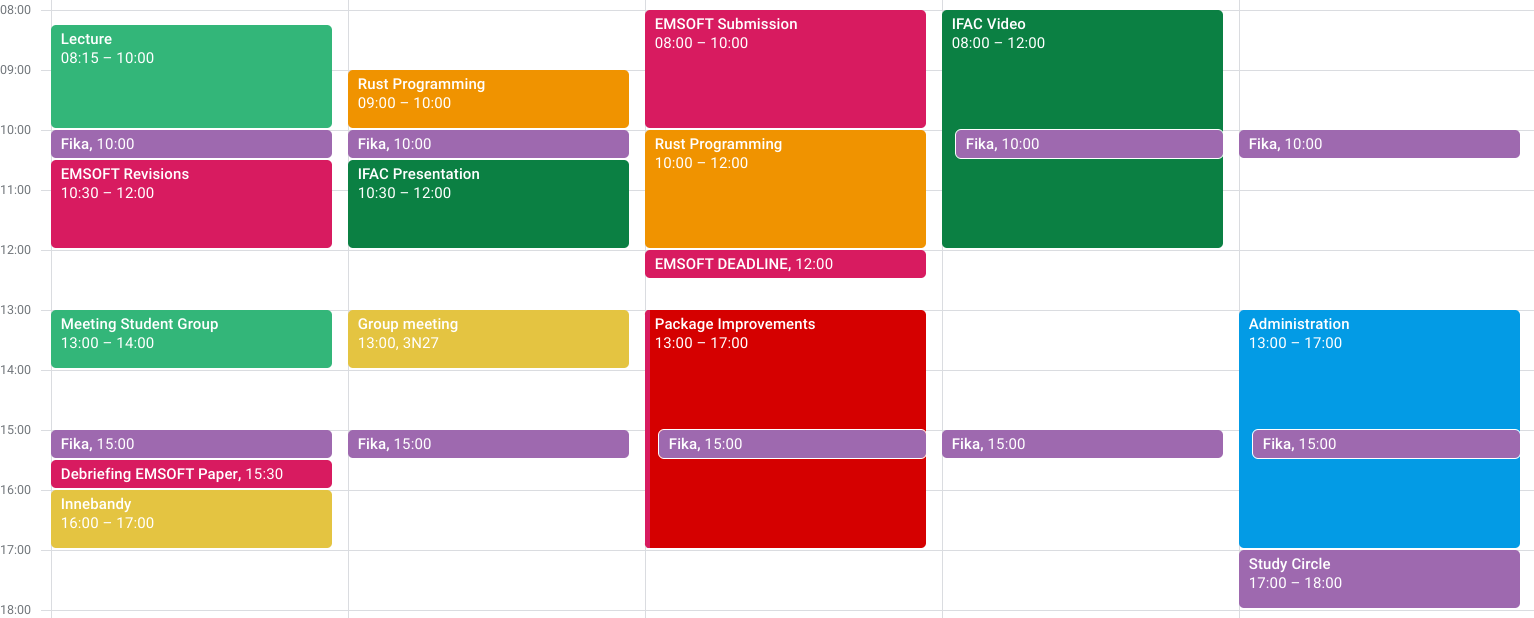
\includegraphics[width=1.0\textwidth]{figs/topic/schedule.png}}%
        \only<2>{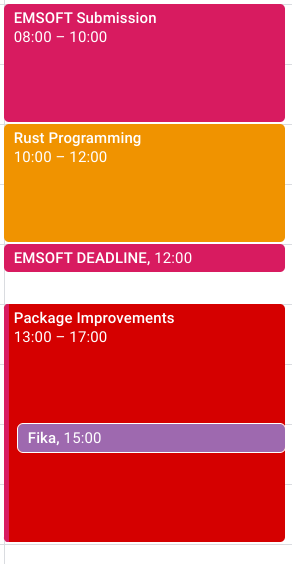
\includegraphics[width=0.25\textwidth]{figs/topic/small-schedule.png}}%
        \only<3>{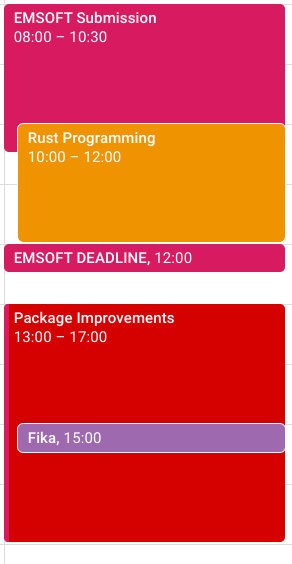
\includegraphics[width=0.25\textwidth]{figs/topic/small-schedule-overrun.png}}
    \end{figure}
\end{frame}

\begin{frame}
    \frametitle{Computational Flow}%
    \framesubtitle<1>{Kill + Zero}%
    \framesubtitle<2>{Kill + Hold}%
    \framesubtitle<3-4>{Skip}%
    \begin{minipage}{0.49\textwidth}
        \only<1>{%
            \begin{tabular}{l l}
                Kill: & Job termination; Revert all progress\\
                & \\
                Zero: & No output
            \end{tabular}
        }%
        \only<2>{%
            \begin{tabular}{l l}
                Kill: & Job termination; Revert all progress\\
                & \\
                Hold: & Same output as previous job
            \end{tabular}
        }%
        \only<3>{%
            \begin{tabular}{l l}
                Skip: & Terminate next job\\
                & \\
                Zero: & No output
            \end{tabular}
        }%
        \only<4>{%
            \begin{tabular}{l l}
                Skip: & Terminate next job\\
                & \\
                Hold: & Same output as previous job
            \end{tabular}
        }%
    \end{minipage}\hfill
    \begin{minipage}{0.49\textwidth}
        \begin{figure}[h]
            \centering
            \only<1-2>{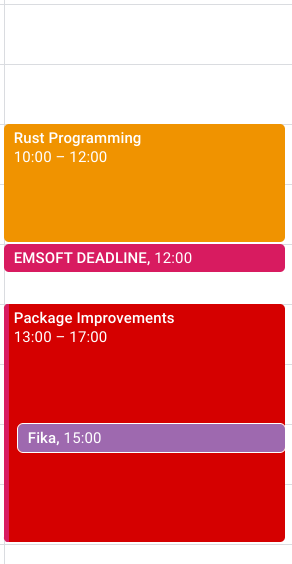
\includegraphics[width=0.5\textwidth]{figs/topic/small-schedule-kill.png}}%
            \only<3-4>{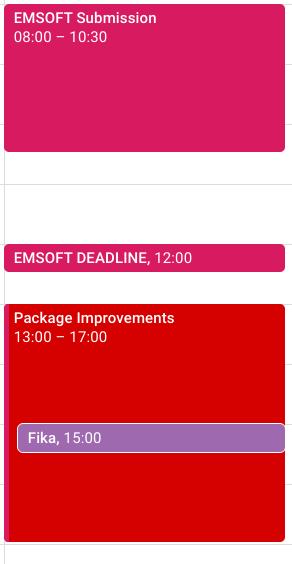
\includegraphics[width=0.5\textwidth]{figs/topic/small-schedule-skip.png}}
        \end{figure}
    \end{minipage}
\end{frame}

\begin{frame}
    \frametitle{Computational Overrun Models}
    \setbeamercovered{transparent}
    \begin{itemize}\setlength\itemsep{1em}
        \item \textcolor<2>{hicolour!50!white}{Soft -- \emph{Probabilistic}\footnote{\cite{Buttazzo:2005, Manolache:2004, vonderBrueggen:2021}}}
        \item \textcolor<2>{hicolour}{Firm -- \emph{Constrained}\footnote{\cite{Koren:1995, Bernat:2001}}}
        \item<1> Hard -- \emph{Infallible}\footnote{\cite{Liu:1973}}
    \end{itemize}
\end{frame}

\begin{frame}
    \frametitle{Computational Overrun Models}
    \framesubtitle{The Weakly-Hard Model(s)}
    \begin{minipage}[c]{0.24\textwidth}
        \centering
        \begin{equation*}
            \begin{matrix}
                {\Large \anyhit{}}   \\
                            \\
                \tAH{}
            \end{matrix}
        \end{equation*}
    \end{minipage}\hfill
    \begin{minipage}[c]{0.24\textwidth}
        \centering
        \begin{equation*}
            \begin{matrix}
                {\Large \anymiss{}}   \\
                            \\
                \tAM{}
            \end{matrix}
        \end{equation*}
    \end{minipage}\hfill
    \begin{minipage}[c]{0.24\textwidth}
        \centering
        \begin{equation*}
            \begin{matrix}
                {\Large \rowhit{}}   \\
                            \\
                \tRH{}
            \end{matrix}
        \end{equation*}
    \end{minipage}\hfill
    \begin{minipage}[c]{0.24\textwidth}
        \centering
        \begin{equation*}
            \begin{matrix}
                {\Large \rowmiss{}}   \\
                            \\
                \tRM{}
            \end{matrix}
        \end{equation*}
    \end{minipage}

    \vspace{1cm}

    \only<1>{\begin{equation*}
        \ldots\, 0\, 1\, 1\, 1\, 0\, 1\, 0\, 1\, 1\, 1\, 0\, 0\, 1\, 1\, 1\, 0\, 1\, 0\, 1\, 1\, 0\, 0\, 1\, 1\, 0\, 1\, 1\, 0\, 1\, 1\, 1\, 1\, 1\, 0\, \ldots
    \end{equation*}
    \vspace{1em}
    \centering
    \phantom{\textcolor{red}{$0$} = Overrunning the deadline}
    }%
    \only<2>{\begin{equation*}
        \ldots\, 0\, \textcolor{hicolour}{1\, 1\, 1\, }0\, \textcolor{hicolour}{1\, }0\, \textcolor{hicolour}{1\, 1\, 1\, }0\, 0\, \textcolor{hicolour}{1\, 1\, 1\, }0\, \textcolor{hicolour}{1\, }0\, \textcolor{hicolour}{1\, 1\, }0\, 0\, \textcolor{hicolour}{1\, 1\, }0\, \textcolor{hicolour}{1\, 1\, }0\, \textcolor{hicolour}{1\, 1\, 1\, 1\, 1\, }0\, \ldots
    \end{equation*}
    \centering
    \vspace{1em}
    \textcolor{hicolour}{$1$} = Meeting the deadline}%
    %
    \only<3>{\begin{equation*}
        \ldots\, \textcolor{red}{0\, }1\, 1\, 1\, \textcolor{red}{0\, }1\, \textcolor{red}{0\, }1\, 1\, 1\, \textcolor{red}{0\, 0\, }1\, 1\, 1\, \textcolor{red}{0\, }1\, \textcolor{red}{0\, }1\, 1\, \textcolor{red}{0\, 0\, }1\, 1\, \textcolor{red}{0\, }1\, 1\, \textcolor{red}{0\, }1\, 1\, 1\, 1\, 1\, \textcolor{red}{0\,} \ldots
    \end{equation*}
    \vspace{1em}
    \centering
    \textcolor{red}{$0$} = Overrunning the deadline}%
    %
    \only<4>{\begin{equation*}
        \ldots\, 0\, 1\, 1\, 1\, 0\, 1\, 0\, 1\, 1\, 1\, 0\, \underbracket{0\, 1\, 1\, 1\, 0\, 1\, 0\, 1\, 1}\, 0\, 0\, 1\, 1\, 0\, 1\, 1\, 0\, 1\, 1\, 1\, 1\, 1\, 0\, \ldots
    \end{equation*}}%
    \only<5>{\begin{equation*}
        \ldots\, 0\, 1\, 1\, 1\, 0\, 1\, 0\, 1\, 1\, 1\, 0\, 0\, \underbracket{1\, 1\, 1\, 0\, 1\, 0\, 1\, 1\, 0}\, 0\, 1\, 1\, 0\, 1\, 1\, 0\, 1\, 1\, 1\, 1\, 1\, 0\, \ldots
    \end{equation*}}%
    \only<6>{\begin{equation*}
        \ldots\, 0\, 1\, 1\, 1\, 0\, 1\, 0\, 1\, 1\, 1\, 0\, 0\, 1\, \underbracket{1\, 1\, 0\, 1\, 0\, 1\, 1\, 0\, 0}\, 1\, 1\, 0\, 1\, 1\, 0\, 1\, 1\, 1\, 1\, 1\, 0\, \ldots
    \end{equation*}}%
    \only<7>{\begin{equation*}
        \ldots\, 0\, 1\, 1\, 1\, 0\, 1\, 0\, 1\, 1\, 1\, 0\, 0\, 1\, 1\, \underbracket{1\, 0\, 1\, 0\, 1\, 1\, 0\, 0\, 1}\, 1\, 0\, 1\, 1\, 0\, 1\, 1\, 1\, 1\, 1\, 0\, \ldots
    \end{equation*}}%
\end{frame}

\begin{frame}
    \frametitle{How do deadline misses occur?}
    \begin{itemize}\setlength\itemsep{1em}
        \item Interference\footnote{\cite{Stankovic:1995, Bernat:2001}}
        \item Cache Misses\footnote{\cite{Milligan:1996, Wang:2012, Altmeyer:2014, Davis:2013}}
        %\item CPU overloads\footnote{\cite{Baruah:1997, Xu:2015, Ernst:2014}}
        \item Security attacks\footnote{\cite{hashemi2018comparison, sabaliauskaite2017comparison, Knorn:2019}}
    \end{itemize}
\end{frame}

\begin{frame}
    \frametitle{Why should we care?}
    For the most time-critical functions, roughly how frequently can deadlines be missed without causing system failure?~\parencite{Akesson:2020}
    \begin{figure}[h]
        \centering
        \resizebox{0.9\textwidth}{!},
symbolic y coords={%
    {I do not know},
    {Never},
    {$1$ in $1$ million to $1$ in $1$ billion},
    {$1$ in $10\,000$ to $1$ in $1$ million},
    {$1$ in $100$ to $1$ in $10\,000$},
    {$1$ in $10$ to $1$ in $100$},
    {More often than $1$ in $10$},
    {Not a concern}},
ytick=data,
nodes near coords,
nodes near coords align={horizontal},
]
\addplot coordinates {
    (35,{I do not know})
    (15,{Never})
    (9,{$1$ in $1$ million to $1$ in $1$ billion})
    (8,{$1$ in $10\,000$ to $1$ in $1$ million})
    (6,{$1$ in $100$ to $1$ in $10\,000$})
    (17,{$1$ in $10$ to $1$ in $100$})
    (3,{More often than $1$ in $10$})
    (7,{Not a concern})};
\end{axis}
\end{tikzpicture}}

    \end{figure}
\end{frame}
